 



\chapter{The power grid}
%\section{History of the power grid}
%conventional power Grid






\section{The Conventional Power Grid}
The \acrfull{cpg} is described in several papers, and books like \cite{BlumeStevenW2007Epsb}, as  a uni-directional, manually controlled, power distribution system.  

\begin{figure}[ht]
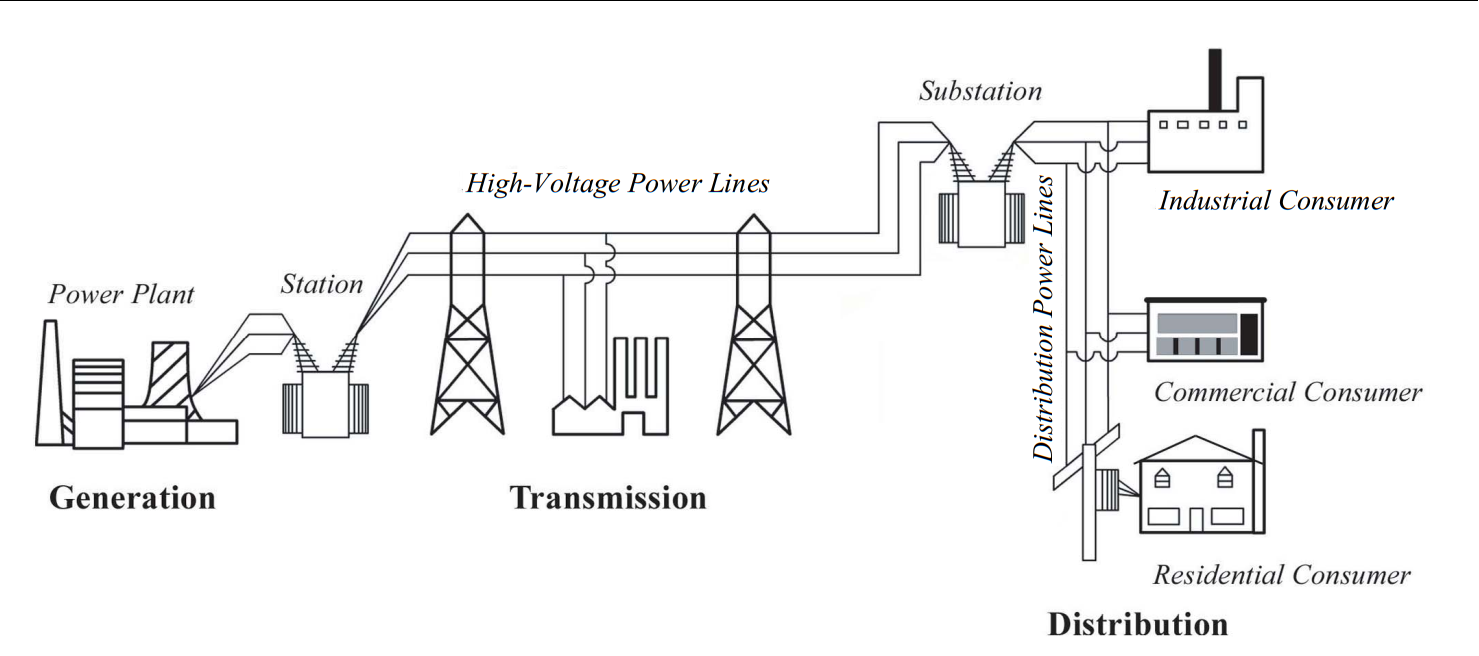
\includegraphics[width=\linewidth]{figures/Blume-PowerGrid-SystemOverView.png}
\caption[Power Grid System Overview]{Power Grid System Overview , as presented in \cite{BlumeStevenW2007Epsb}}
\label{fig:Blume-PowerGrid-SystemOverView}
\end{figure}



\subsection{Overview of the Conventional Power Grid}
The \acrlong{cpg} is a system by which electric power is centrally generated, transmitted, and distributed to industrial, residential,and commercial end users, in order to ensure a reliable access to a sufficient amount of electrical energy. 
\newpage
The \acrlong{cpg}, as described in \cite{BlumeStevenW2007Epsb}, consists of the following subsystems:

\begin{itemize}

 \item The \textbf{Generation Subsystem} which Generates electric power from various sources of energy, to be transmitted for distribution to Consumers. Some examples of installations generating electrical power are nuclear power plants, as well as hydroelectric power plants, feeding water-driven turbines in order to generate power.
 \item The \textbf{Transmission Subsystem} which transmits electric power from the Generation subsystem to the Distribution Subsystem. The current is transmitted via high voltage power lines, minimising energy loss over longer distances.
 \item The \textbf{Distribution Subsystem} which distributes electric power to end users, after converting the high voltage input into lower voltage levels, suitable for consumption.
 \end{itemize}

As described in Chapter 2.3 of \cite{Rihan2018} %\cite{SmartGridOverview2013}
, the \acrlong{cpg} is facing challenges, related to Black Outs adhering to the increased demands for electrical power . 


%\section{The Smart Grid}
%smart Grid
\section{The Smart Grid}




In order to provide a description of the \acrfull{sg}, a description of the characteristics of the \acrlong{cpg} is provided.





As described in  \cite{BlumeStevenW2007Epsb} by \citeauthor{BlumeStevenW2007Epsb}, some of the characteristics of the \acrlong{cpg} are:

\begin{itemize}
\item Power is generated in real time. In the event a consumer is "flipping a power switch," the power grid must have sufficient resources in order to keep the voltage levels at an acceptable level.
\item The \acrlong{cpg} is controlled by a central management facility known as the \acrfull{scada} subsystem. The monitoring and management of the \acrshort{pg} is initiated from the Control Center, utilising unidirectional communication channels. 
\item The \acrlong{cpg} \acrlong{scada} subsystem is offline, i. e. not connected to any publicly available network. Therefore, operational duties must be performed by personnel physically located at dedicated operational sites.

\end{itemize}

The \acrlong{cpg} originates from the local society-serving power generation facilities initiating the supply of electrical power, which over the years were interconnected to form a grid, connecting consumers to a network of several power generating facilities, providing a more flexible power distribution infrastructure. 


\subsection{Overview of The Smart Grid}


The \acrfull{nist} has published a \hl{conceptual} model of the smart grid, as shown in 
figure \ref{fig:NIST-SmartGRID-ConceptualModel}.



\begin{figure}[ht]
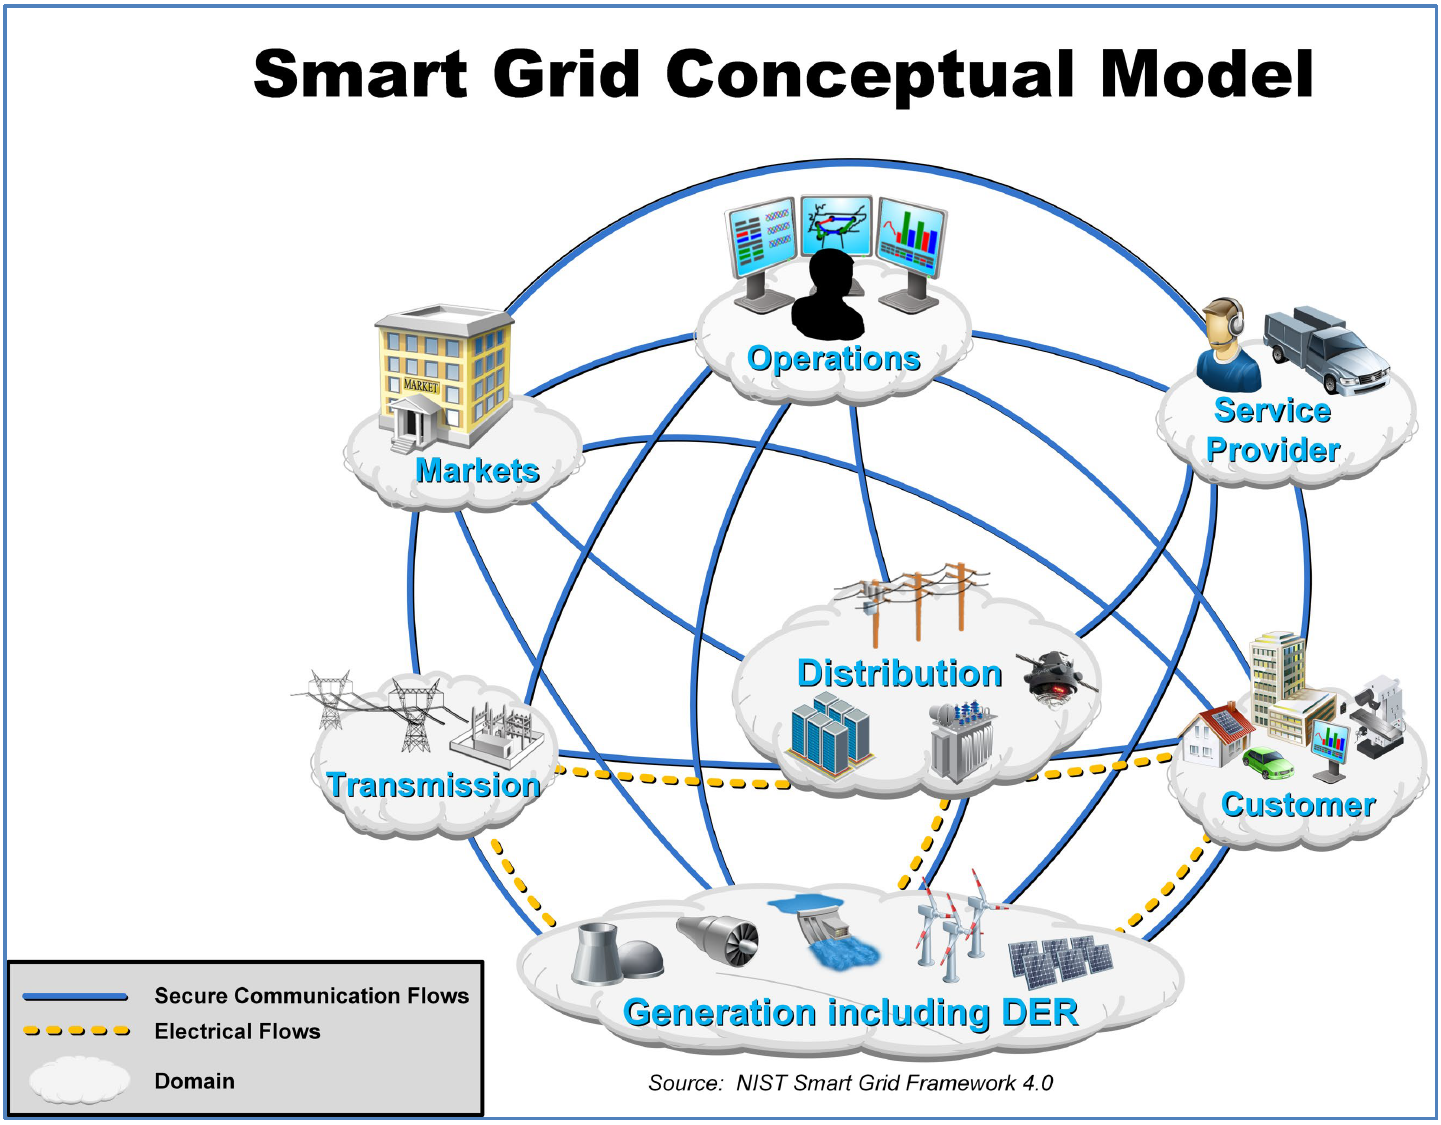
\includegraphics[width=\linewidth]{figures/NIST-SmartGRID-ConceptualModel.png}
\caption[Smart Grid Conceptual Model]{Updated \acrlong{sg} conceptual model, as presented in \cite[p. 13]{gopstein2021nist}, Figure 4}
\label{fig:NIST-SmartGRID-ConceptualModel}
\end{figure}






The \acrlong{sg} adds Information and Communication Technology (ICT) to the \acrlong{cpg}, in order to transform the  unidirectional communication lines of the monitoring and control infrastructure of the \acrlong{cpg}, into an infrastructure utilising two-way communication between the various parts of the \acrlong{sg} infrastructure. 






%\subsection{The Smart Grid: Critical Information Infrastructure}
%According to \cite[p. 610]{Bîrleanu2019}, the \acrlong{sg} consists of the following subsystems:

%\begin{itemize}
%\item \textbf{the conventional  power grid}
%\item \textbf{intelligent equipment} 
%\item \textbf{communication infrastructure}
%\end{itemize}

%\cite{Bompard2012}...

%...\acrlong{sg} Subsystems
%\begin{itemize}
%\item 
%\end{itemize}




\subsection{The Smart Grid Domains}




The \acrshort{sg} consists of seven domains, as shown in \figureautorefname { }\ref{fig:NIST-SmartGRID-ConceptualModel}:


    \subsubsection{Customer Domain} The customers are the Consumers of Electricity.
    The power infrastructure of commercial or private customers includes \acrfull{ami}, monitoring the amount of energy consumed, both for billing and \acrfull{dr} purposes. Consumers may plan their consumption, avoiding high-cost periods of heavy load, by  selecting time frames of low prices.
    \subsubsection{Markets Domain} The participants of the Markets Domain aims to balance the consumption and demand of electricity, by adjusting prices on electricity. Price adjustments may be used in order to shift consumption from periods of high demand, to periods of low demand.     
    \subsubsection{Service Provider Domain} Services to the Customers,  as well as the Markets and Operators domain, are provided by the Service Provider Domain, fulfilling duties like customer management and billing, as well as a number of emerging services as required. 
    \subsubsection{Operations Domain} This domain consists of Electricity service operators, ensuring efficient and fail-safe \acrfull{sg} operation, by utilising \acrshort{scada} systems and \acrlong{ems}s in order to monitor and control system operational state.  
    \subsubsection{Bulk Generation Domain} The facilities for producing electricity, resides in this domain. In addition to the connection and interaction with  to the Transmission domain, it interacts with the Markets domain, as well as the operations domain.  
    \subsubsection{Transmission Domain} The actors of the Transmission domain aims to reduce energy loss while transmitting a stable and reliable stream of energy from operators in the bulk generation domain to the distribution domain. The market domain provides input on expected level of demand which may require adjustments of the amount of electricity distributed, controlled and monitored by actors in the operation domain.  
    \subsubsection{Distribution Domain} The actors of the Distribution Domain delivers the electricity to consumers according to demand and availability, and monitors generation and consumption data. Bi-directional power-flow is supported. In the case customers have private  power producing facilities, like solar cells and wind turbines, any surplus electricity might be sold, and distributed to other customers.



The authors of \cite{uslar2019applying}, \citeauthor{uslar2019applying} describes an alternative model for the \acrshort{sg}, originating from , and visualised in figure \ref{fig:SGAM}. The model consists of three dimensions, named "Domains", "Zones", and the "Interoperability dimension". 

\begin{figure}[ht]
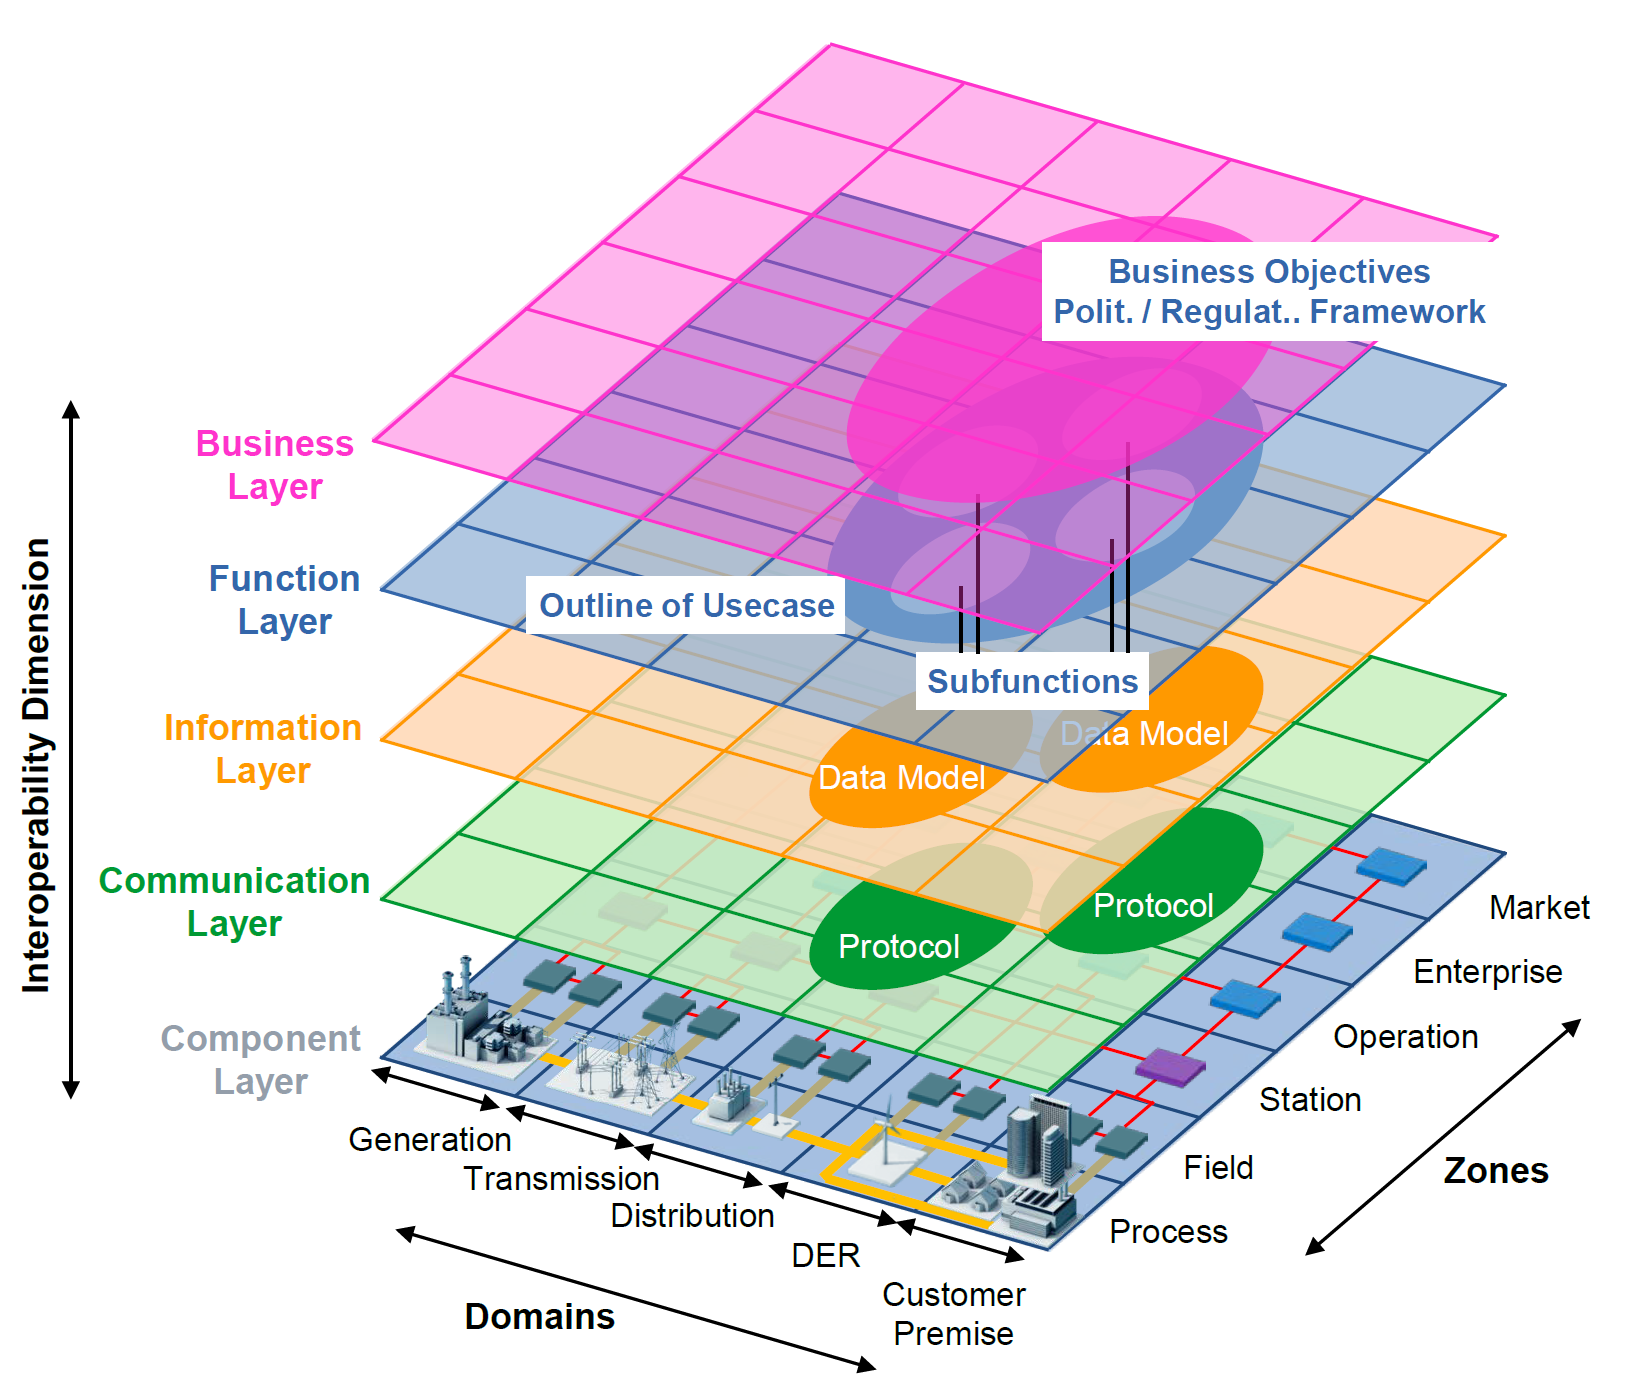
\includegraphics[width=\textwidth]{figures/SGAM.png}
\caption[SGAM Smart Grid Model]{SGAM Smart Grid Model , as presented in \cite{uslar2019applying}}
\label{fig:SGAM}
\end{figure}

The "Domains" dimension consists of the following domains:

\begin{itemize}
    \item The \textbf{Generation} domain:
    \item The \textbf{Transmission} domain:
    \item The \textbf{Distribution} domain:
    \item The \textbf{DER} domain:
    \item The \textbf{Customer Premise} domain:
\end{itemize}




\section{Protocols}
A large number of protocols are defined, in order to standardise the operation of the \acrlong{sg}.

A small selection of these, relevant for the scope of the thesis, are described underneath.

\cite{2021arXiv210311657E} \hl{describes communication protocols} in the  \acrshort{sg}.





The \acrshort{sg} consists of a vast number of both conventional and modern, more dynamic, production facilities, which requires thorough monitoring in order to ensure the optimal distribution of electrical energy. The requirement of a consistently stable and reliable supply of energy is constant, while the amount of energy demanded is dynamically changing according to the demand for power at any time. \\ 

Therefore, the proper \acrshort{sg} operation might be considered virtually impossible without a  close monitoring of current power flow, as well as the ability to instantly adjust the supply of power according to present needs,  without the risk of causing power surges or blackouts. For this purpose, the Wide Area Monitoring System analyses the levels of electrical power as monitored by sensors, synchronised according to a common GPS-controlled time source. \\ 

The correctness of this time source is critical to the reliability, and therefore, the proper operation of the monitoring system, constituting the primary decision criteria for actions controlling the supply of power.


